\chapter{Decision Trees {\color{red} DRAFT} \label{chapter:decisiontrees}}

{\bf Decision trees} were developed as an alternative to neural networks in the 1970s. They can be used either for classification or regression. There are several algorithms for fitting decision trees, all of which are heuristic, because the general problem of learning an optimal decision tree for a dataset is NP-complete. All algorithms for tree learning are \textbf{greedy} and are not guaranteed to give the optimal solution.

\subsection{Entropy and Information Gain}

Today we will discuss the ID3 algorithm for building decision trees, which relies on the concepts of entropy and information gain. \textbf{Entropy}, usually abbreviated $H$, is a measure of the uncertainty in the value of a random variable. It is the number of bits (on average) required to describe the outcome of the random variable. Here is the formula for the entropy of the discrete probability distribution governing the outcome of a random variable, $X$:

$$ H(X) = - \sum_{x} P(X = x) \log_2\left(P(X = x)\right) $$

For a Bernoulli random variable, there are only two possible outcomes: 0 and 1. The entropy of this random variable is given by:

$$ H_\text{Bernoulli} = -\mu \log_2(\mu) - (1 - \mu) \log_2 (1 - \mu) $$

where $\mu$, as usual, is the probability the outcome is 1. 

Let $Y$ be the outcome variable of a training set. Let $X$ be some other random variable defined over the training set. It could be one of the original predictors or some arbitrary combination of them. \textbf{Information gain} is defined as:
\begin{align*} \text{Gain}(Y, X) &= H(Y) - \sum_{x} P(X = x)~ H(Y|X=x) \\
&= H(Y) - H(Y|X) \end{align*}
It is a measure of how much our uncertainty in the value of $Y$ is reduced by knowing $X$. 

\subsection{The ID3 Algorithm}

Here is the algorithm:
\begin{enumerate}
\item Start with a single node representing the entire dataset.
\item At each current leaf node in the tree:
\begin{enumerate}
\item Compute the information gain for each feature in turn.
\item Split on the one with the highest information gain.
\end{enumerate}
\item Return to Step 2. Stop the recursion when either the class distributions at the leaf nodes are entirely pure (all data points at a leaf have the same outcome class), or there are no more variables left to split on.
\end{enumerate}

\subsection{Decision Tree Regression}

So far we've assumed that our outcome is discrete. But what happens if it's numeric? (That is, what if we want to perform regression instead of classification?)

In that case, we use \textbf{standard deviation reduction} instead of information gain to decide which variables to split on. The sample standard deviation of an outcome, $y$, is defined as:

$$ S(Y) = \sqrt{\frac{\sum_i(y^{(i)} - \overline{y})}{n-1}} $$

The procedure is identical to the ID3 algorithm except you use conditional standard deviation instead of information gain to decide on features. We define

$$ S(Y, X) = \sum_{x} P(X = x)~ S(Y(X=x)) $$

and at each current leaf node, we split on the variable where the reduction in standard deviation, $S(Y) - S(Y,X)$, is the highest. 

\subsection{Numeric Predictors}

So far we've also assumed that our predictors are discrete. But decision trees can handle numeric predictors as well. There are many different strategies for deciding on an optimal split for a predictor. Two simple ones:

\begin{itemize}
\item Split at the median or mean of the predictor.
\item Order the datapoints on the value of the predictor and consider each possible split, looking for the one that gives the greatest information gain/standard deviation reduction. So for example, if you have a predictor called ``age'' and its values are $10, 11, 16, 18, 20$, and $35$, consider all $N-1 = 5$ possible split points. (This is the approach used by C4.5, a successor to ID3.) 
\end{itemize}

If you have a large dataset, the second option is probably not practical, but you can downsample your dataset first and then look for the optimal cut point(s).

What if the outcome is numeric? In that case, we can use \textbf{standard deviation reduction} instead of information gain to decide which variables to split on. The sample standard deviation of an outcome, $y$, is defined as:
$$ S(Y) = \sqrt{\frac{\sum_i(y^{(i)} - \overline{y})^2}{n-1}} $$
where $\overline{y}$ is the overall mean of the outcome. The procedure is identical to the ID3 algorithm (see Chapter~\ref{chapter:decisiontrees}) except you use conditional standard deviation instead of information gain to decide on features. We define
$$ S(Y, X) = \sum_{x \in \text{Values(X)}} \frac{|Y(X=x)|}{|Y|}~ S(Y(X=x)) $$
and at each current leaf node, we split on the variable where the reduction in standard deviation, $S(Y) - S(Y,X)$, is the highest.

For example, imagine you had a dataset similar in structure to our example, but instead of two real-valued predictors, you have two binary predictors, $x_1$ and $x_2$. The decision tree algorithm could choose either one of them to split on first. Here are the distributions of outcome values associated with $x_1$ and $x_2$. 

\begin{center}
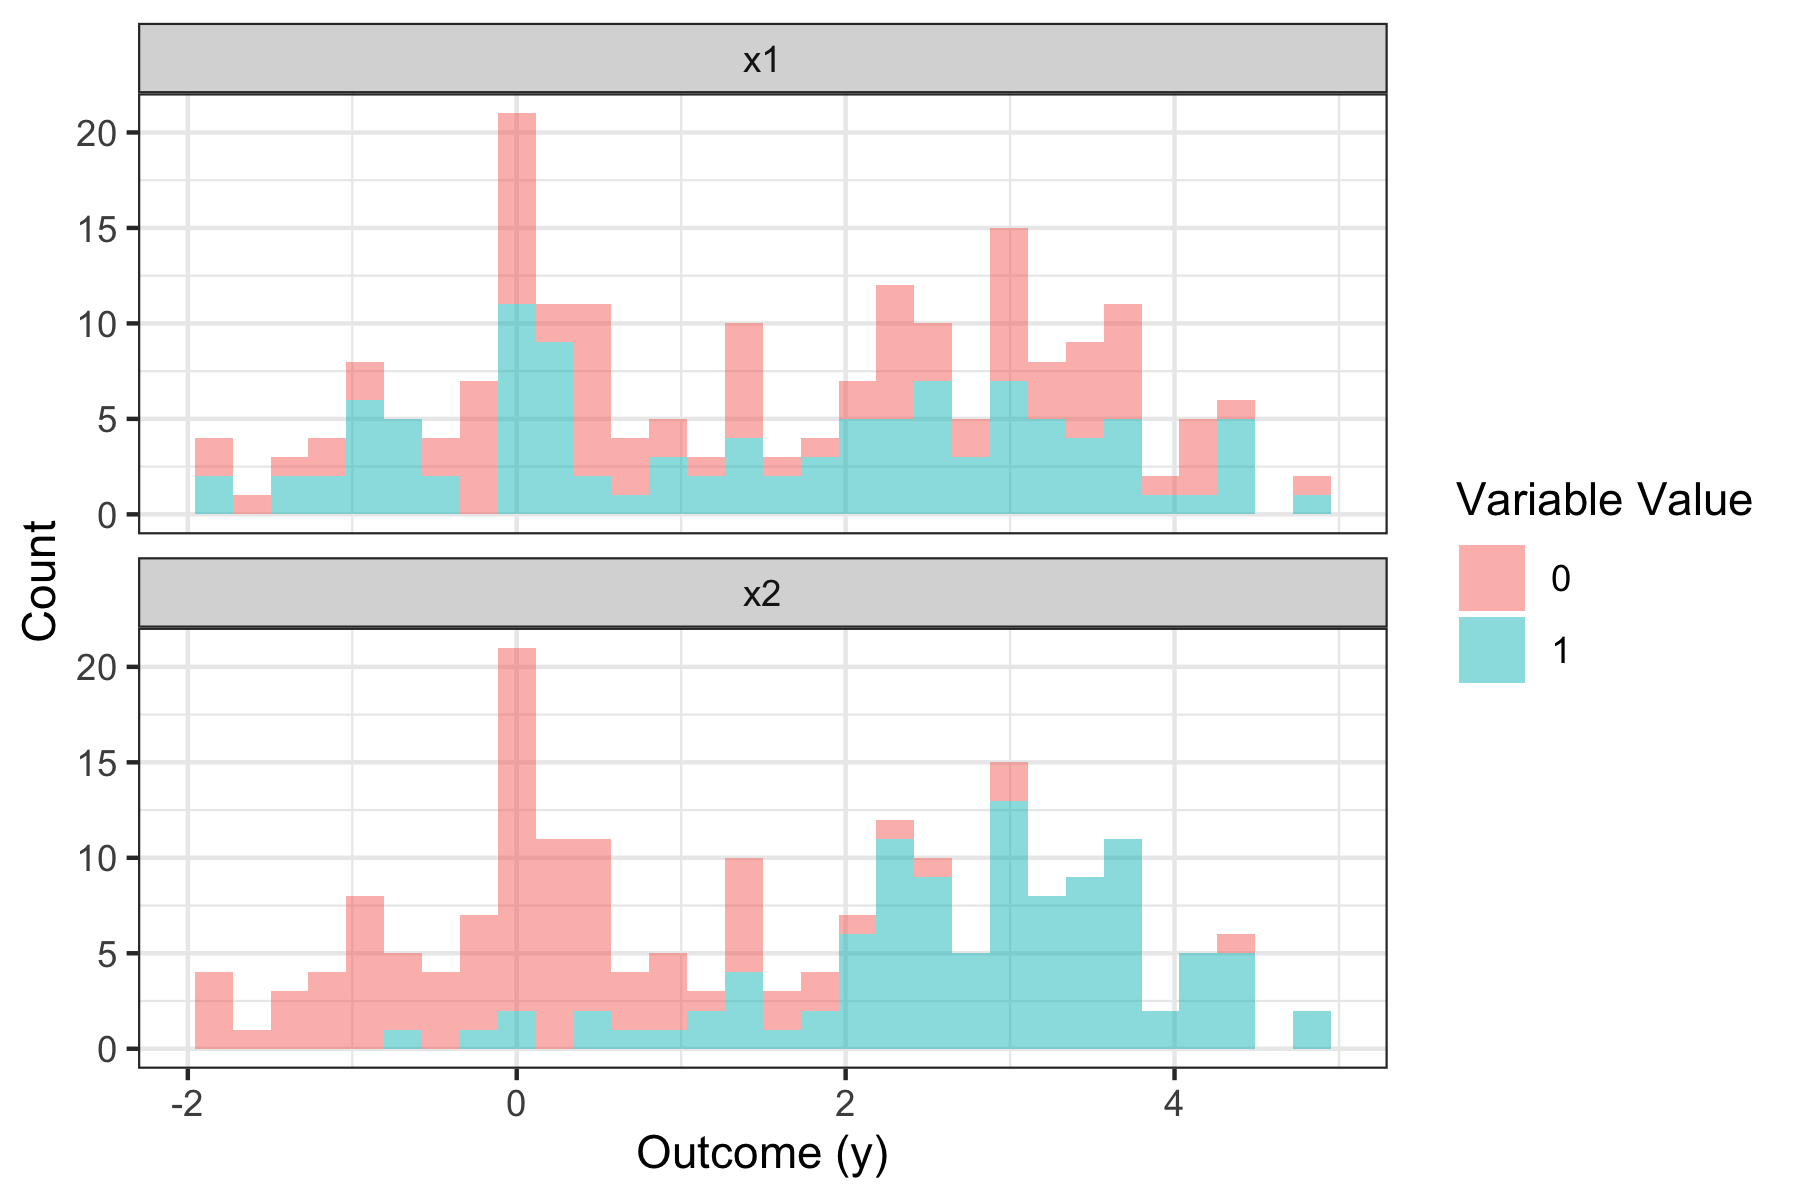
\includegraphics[width=0.9\textwidth]{img/esl-reg-decision-tree-varsplit.png}
\end{center}

\begin{question}{}
Which of these two variables, $x_1$ or $x_2$, would make the most sense for a decision tree to split on? What would such a split look like and what would the output value of the tree (the predicted value of $y$) be for each side of the split?
\end{question}

